%%%% imav.tex
% This is the tex-file for the IMAV 2014 conference
% for questions / remarks / bugs regarding the files, please contact info@imavs.org
% You can use this style for your conference, as long as you refer to the IMAV 2014
% in a comment similar to this one.
% Of course, the IMAV 2014 is not liable for any aspects of its use.

\documentclass{article}
% The style file
\usepackage{imav}
% Use the postscript times font!
\usepackage{times}
\usepackage{graphicx}
\usepackage{algorithm}
\usepackage{algorithmic}
\usepackage{wasysym}
\usepackage{color}
%\numberwithin{algorithm}{chapter}
%\usepackage{algorithmicx}
% the following package is optional:
\usepackage{latexsym}

\usepackage [english]{babel}
\usepackage [autostyle, english = american]{csquotes}
\MakeOuterQuote{"}

\usepackage{acronym}


\title{Autonomous Flight of Micro Air Vehicles 2015 - Group 6}
\author{M. Bevernaegie\thanks{M.Bevernaegie@student.tudelft.nl}, C. Cheung\thanks{C.Cheung@student.tudelft.nl}, Y.I. Jenie\thanks{Y.I.Jenie-1@tudelft.nl}, S.H. Lee\thanks{S.H.Lee-2@student.tudelft.nl}, P. Lu\thanks{P.Lu-1@tudelft.nl} \\ Delft University of Technology, Delft, The Netherlands}

\begin{document}

\maketitle

\begin{abstract}
{\color{red} This should be done at the end - by Cherry}
\end{abstract}

\section{Introduction} \label{section:introduction}
This report is structured as follows. In the end of this introduction, three main equipments for the project is introduced. Section 2 follows with the explanation of the vision algorithm used to achieve the goal of the project. Our Drone flight-plans are elaborated in section 3 by comparing two possible plans our team came up with. Two types of simulation were conducted before the tournament, elaborated in Section 4 along with the result analysis. The competition result, as well as the discussion, follows in section 5. Section 6 finally wrap the report with few concluding remarks.

\subsection{AR Drone: A Quad-rotor MAV}
A Quad-rotor named AR Drone 2.0 is the chosen MAV in this project. The first version of the vehicle was build by the Parrot company (France) in 2004, and released for public in 2010, aiming for the market of video games and home entertainment\cite{Bristeau:11}. The platform of the vehicle is a Quad-rotor, a four fixed propeller that are rotated by four brushless motors, each controlled by an ATMEGA8L 8bit microcontroller. The AR.Drone is equipped with 3 cells battery that supplies 11.1 V and 1000 mAh providing power for 10 to 15 minutes of flight. The platform is very popular in MAV research field\cite{Bristeau:11}\cite{Pestana:13}\cite{Lugo:14}, since it has the capability of both hovering and fast forward cruising. In order to make the vehicle acceptable for public, a very effective control and stabilization system is mandatory for a easy piloting platform. The general view of the AR Drone 2.0, the one used for this project, is shown in Figure~\ref{f:TheDrone} below.

\begin{figure}
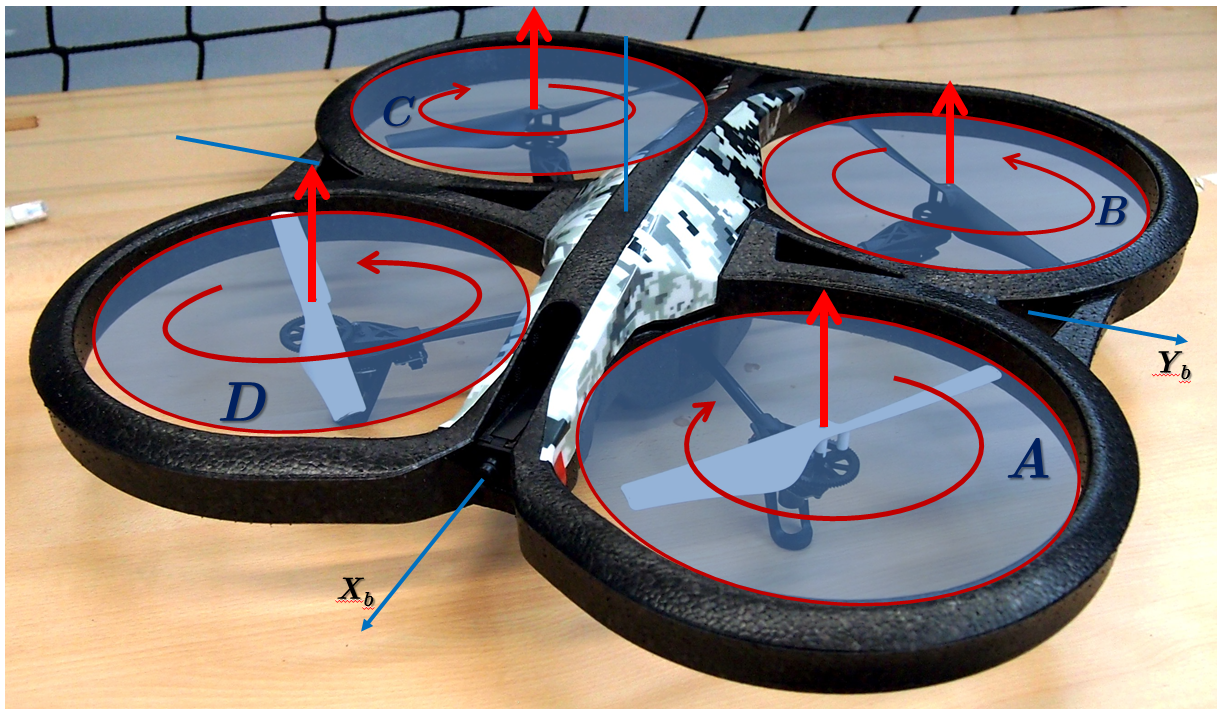
\includegraphics[width=1\linewidth]{Figures/TheDrone.png}
\centering
\caption{The AR Drone 2.0 from the Parrot Inc (France) - with schematic of the four propellers direction of rotation}
\label{f:TheDrone}
\end{figure}

Quad-rotor is controlled by adjusting the thrust and rotation combination of its propellers. AR Drone propeller setup is as shown in Figure~\ref{f:TheDrone}, where two of the propeller (A and C) turn clockwise, while the other two (B and D) turn counter clockwise. On stationary hover condition, every propeller produce the same thrust from the same RPM. Torque from each motor, therefore, are canceled by the combination of propeller rotation. To have a positive pitching motion, more power is given to propeller B and C, while reducing power in A and D to keep the balance with the weight and the desired forward/backward speed. Rolling motion is controlled in similar manner, positive rolling is achieved by giving more power to A and B, while reducing power in C and D. Finally, positive yawing is controlled by giving more power to propeller A and C, while reducing power in B and D. Controlling task for stability is challenging, because the rotational motion, i.e, roll, pitch and yaw, and the translational motions, i.e., heave, sway, and surge, are coupled. The work of \cite{Bouabdallah:07} elaborated this challenge comprehensively.

The Guidance, Navigation, and Control system of AR.Drone is supported by an a set of sensory system consisting a 3-axis accelerometer, a 2-axis gyroscope, a 1-axis gyroscope, and two ultrasonic sensors. The ultrasonic sensor is used for altitude and vertical displacement estimation, while the other is part of an Inertial Measurement Unit (IMU) that is essential for control and stability of the vehicle.All the sensors is chosen to be as low-cost as possible, which implies that the embedded control system have to deal with a lot of bias, misalignment angles, and other errors\cite{Bristeau:11}. Furthermore, two cameras are equipped in AR.Drone, which are not mainly intended to be used as sensor for the flight. Coupled with the IMU rotation measurement and vision algorithms (explained in the next section), however, the camera can be used in vertical speed estimation (camera pointed down). 

\subsection{CyberZoo and OptiTrack}
At march the 5th, 2014, TU Delft's so called \textbf{Cyber Zoo} is opened as a new research and test laboratory for robots and unmanned vehicles. Initiated by the TU Delft Robotic Institute, this facility is a 10 x 10 meters area covered by 7 meter high net. The facility is located in the hangar of the Faculty of Aerospace Engineering, and it is the designated field in which the project MAV will be flown.

The Cyberzoo is equipped with a three dimensional optical motion tracking system based on called OptiTrack by NaturalPoint Inc\cite{Hansen:14}\cite{Guadarrama-Olvera:14}. The system consist of 24 camera, observed in Figure~\ref{f:OptiTrackCyberZoo},  to triangulate the position of retro-reflective markers, placed on the surface of a motion platform in a specific distance between each other, such as shown in Figure~\ref{f:Markers} below. By defining a set of marker positions as a rigid body, the OptiTrack system can recognized the particular pattern and track the motion continuously in a screen, also shown in Figure~\ref{f:OptiTrackCyberZoo}. The OptiTrack then provide, through a UDP connection, a local positioning data that is almost similar with the data provided by a GPS. with the This OptiTrack system is known to be a low-cost system that have accuracy comparable with its more high end competition, the well established Vicon motion capture system\cite{Hansen:14}.

\begin{figure}[h]
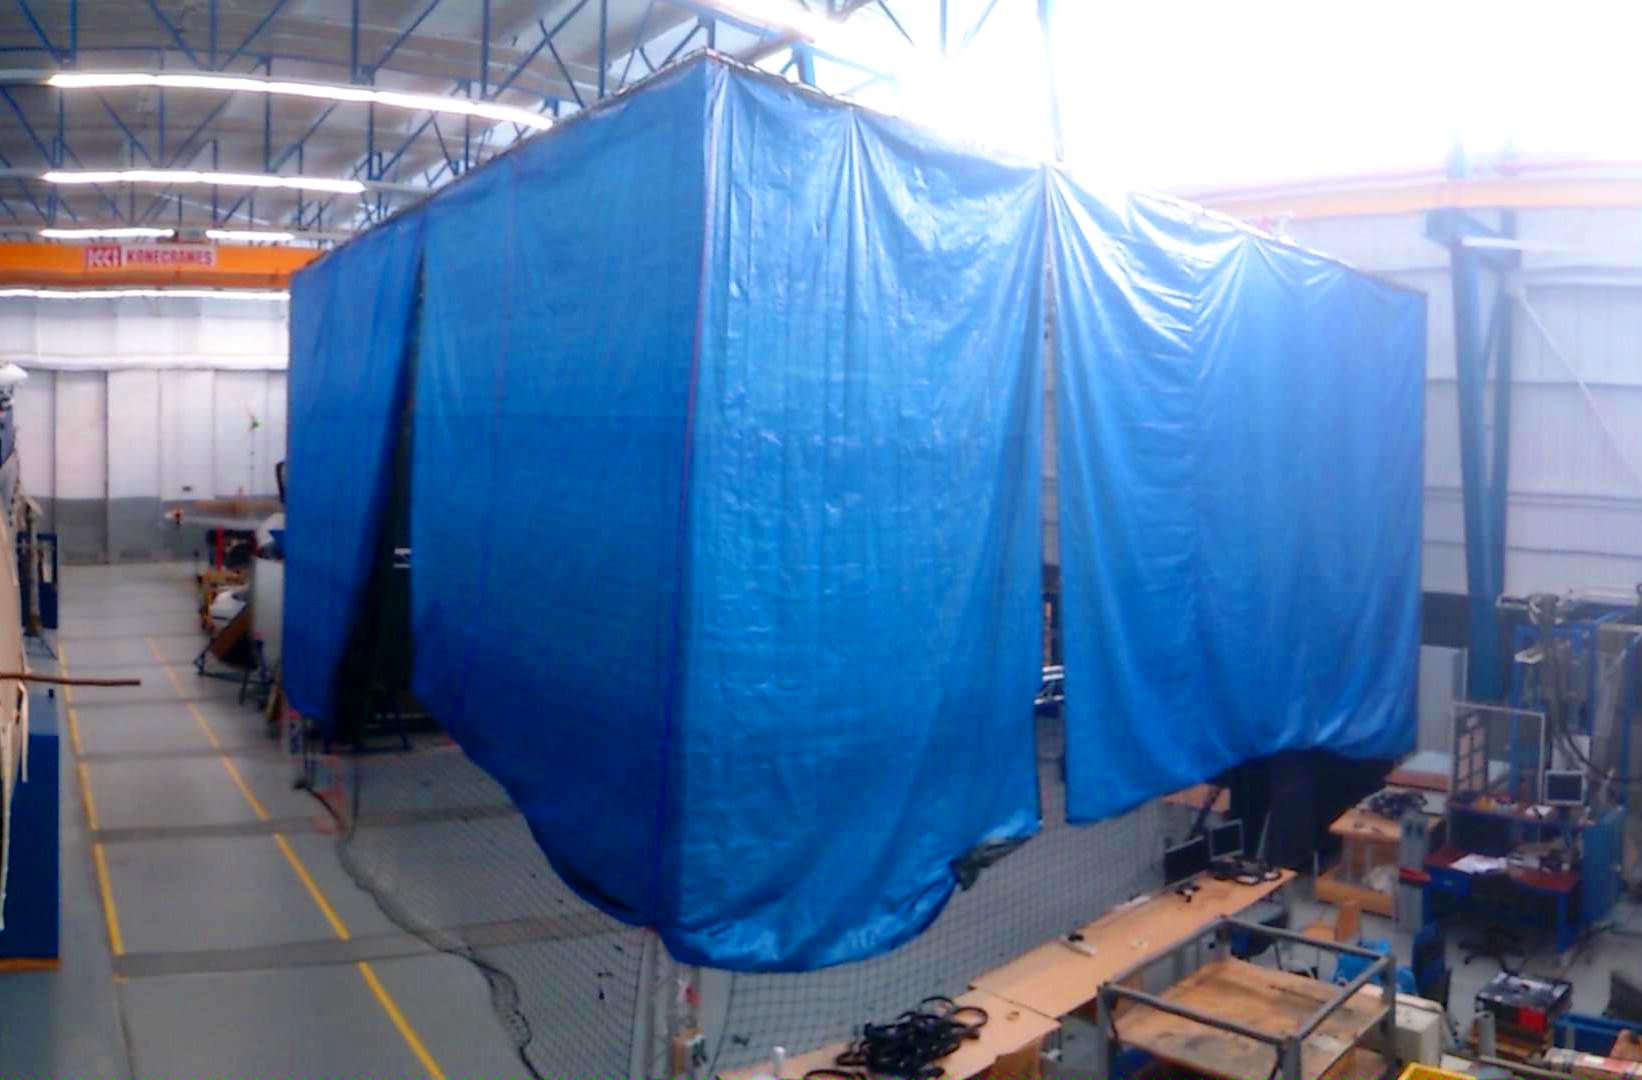
\includegraphics[width=0.9\linewidth]{Figures/TheCyberZoo.png}
\centering
\caption{The cyber zoo inside the hangar of the Faculty of Aerospace Engineering, Delft University of technology. Currently covered by a thick canvas that serves as a background for computer vision for the robots inside}
\label{f:TheCyberZoo}
\end{figure}

\begin{figure}[h]
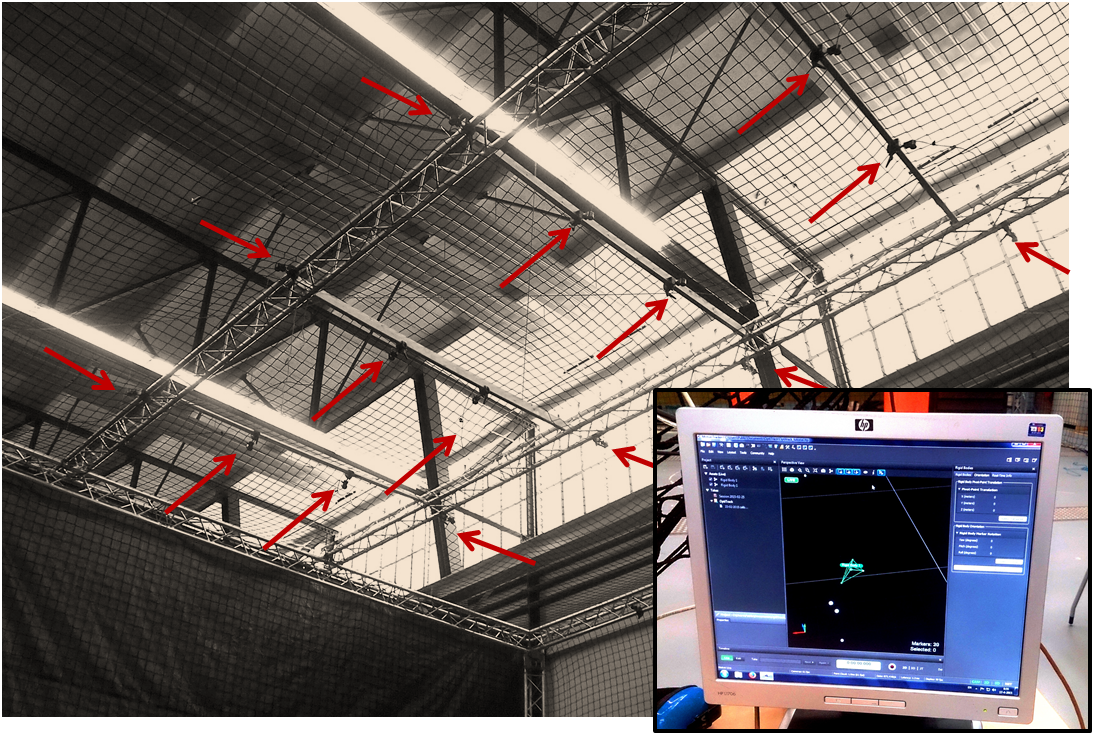
\includegraphics[width=0.9\linewidth]{Figures/OptiTrackCyberZoo.png}
\centering
\caption{Some camera positions on the roof of the cyber zoo. (inset) the OptiTrack GUI that combines data from the 24 camera to triangulate marker positions inside the cyberzoo}
\label{f:OptiTrackCyberZoo}
\end{figure}

\begin{figure}[h]
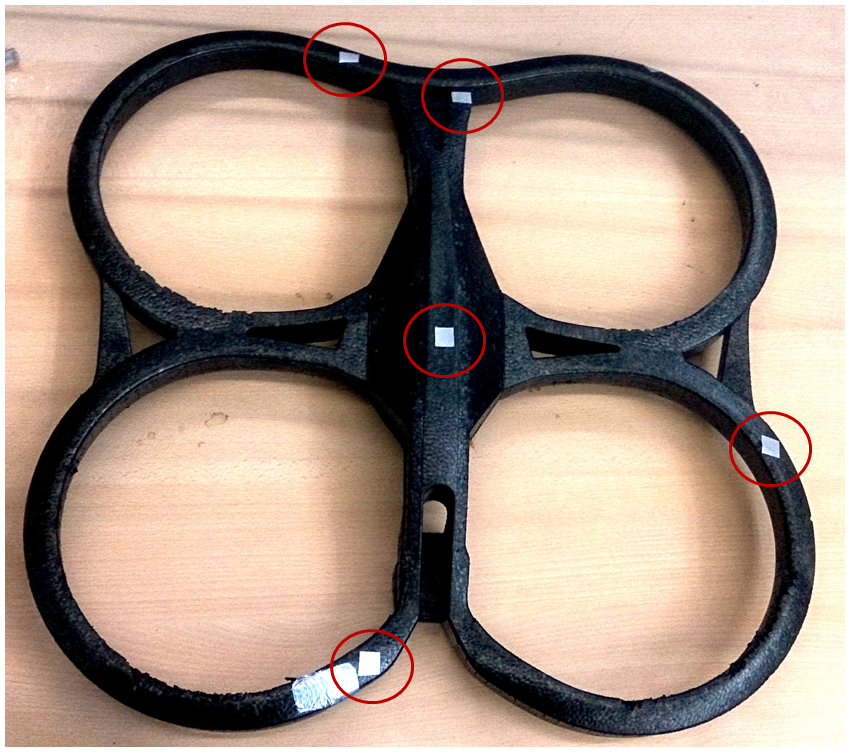
\includegraphics[width=0.7\linewidth]{Figures/Markers.png}
\centering
\caption{Retro-reflective marker is installed on the surface of AR.Drone hull. Each Hull have a specific position combination that can be recorded and tracked by the OptiTrack system}
\label{f:Markers}
\end{figure}

\subsection{Paparazzi: Open Source Autopilot}
The AR.Drone in this project will be equipped with the open source autopilot system Paparazzi, which is mainly developed and maintained by the Ecole Nationale de l'Aviation Civile (ENAC) in Toulousse, France. The system run in a Linux platform, and has been used by hundreds of research from all around the world\cite{Reuder:12}\cite{Royo:11}. The opening window of this software is shown in the Figure below.

%Figure Paparazzi

Paparazzi's Ground Control Station (GCS) is used to determined the flight plan of a vehicle to fly autonomously. The flight plan is mainly set using combination of several blocks, or modules, embedded in the GCS, e.g., the take-off, set direction to a waypoint, go to a waypoint, or go make a circle. A wifi connection is established between Paparazzi and the vehicle for a two-way communications, enabling the AR Drone to sent its states back to the GCS and operator. The flight plans can be interrupted by the operator anytime during the flight.

Inside the cyber zoo, however, the states of position is not given directly by the drone, since it is flying in a GPS-denied environment. Instead, Paparazzi must be modified to receive data from the OptiTrack local positioning. This is done by using the NavNet module in Paparazzi, coupled with a view changes in the airframe and flight plan code. The local position data from each rigid body is sent through a UDP connection, and therefore the computer platform, running Paparazzi in the CyberZoo, is required to have two connection port. 




\section{Vision algorithm}
\subsection{Vision-based Navigation Literature}
\label{subsec:lit_vision}
\textcolor{red}{Here we talk about the vision algorithm used in the literature}
\subsubsection{Optic Flow}
\subsubsection{Computer Vision}
\subsubsection{Mapping} SLAM


\subsection{Own Vision Algorithm}
\label{subsec:our_vision}
In Section \ref{subsec:lit_vision}, a number of the vision-based navigation methods used in literatures were briefly introduced and discussed. Although these methods have shown considerably good results in certain work domains, our team decided to come up with more simple method for the obstacle detection and avoidance. The rationale behind this is as follows:
\begin{itemize}
	\item Lucas-Kanade optic flow generation from Harris corner detector or FAST feature detector will not work well unless the obstacles have many "features" on their surface. In the competition, monotonic orange poles and a black wall will be used, and hence we anticipate that there will not be many features available on the texture of the obstacles.
	\item For the same reason, it will be very difficult to compute the Time-to-Contact because it primarily uses the optical flow vectors.
	\item Object recognition or image classification  method can be difficult for tuning and other practical reasons. For example, in order to avoid the orange poles, one cannot simply judge from the overall color of the image as to whether the obstacle is close enough or not. This is because there are cases where multiple poles are visible in the image, although none of them are close enough to the drone. Also, the poles appearing from the "blind spot" of the camera's view are more likely to be hit than the poles located straight ahead (These are verified during the tests). In comparison to other simpler methods, the object recognition will not allow for a flexible adaption to account for all these various situations.
	\item As the drone has only one front camera, the mapping techniques, such as SLAM, will take considerably more computational time and memory. This technique does not go along well with the objective of the competition which is to enable the drone travel as much as possible while minimizing the collisions.
\end{itemize}

For these reasons, it was necessary to come up with much simpler vision algorithm which can be implemented and tested easily. The proposed vision algorithm uses a simple color thresholding method for the detection of specified obstacles, which is done in the following steps:
\begin{enumerate}
	\item Take only the bottommost row of the pixels in the image as input. Note that the floor will be visible until the distance between the drone and an obstacle standing on the floor becomes lower than a certain threshold distance, assuming that the drone moves slowly in a hovering flight at a fixed altitude. For the visualization, refer to Section \ref{section:simulation}.
	\item By setting a intensity (i.e. Y color channel)  threshold, convert the bottommost pixel row into a binary row which has the elements of value 1 and 0 (i.e. 1 if the pixel intensity value is lower than the threshold, and 0 other wise). Therefore, if the image of the black wall is captured at the bottommost row, it will be indicated by the continuous sequence of 1's.
	\item Count the number of continuous 1's, and if the sequence is longer than a certain threshold, namely the "black wall width-threshold", then mark the position as the position of a black wall. For each mark, give the weight based on the detected width. Determine either to turn left or right, depending on the weighted position of the black wall. 
	\item If there is no black wall detected (i.e. no continuous sequence of 1's exceeding the "black wall width threshold"), evaluate the Cr chroma value to detect the orange poles. Generate a binary row in the similar manner as for the black wall detection by setting an appropriate Cr threshold. 
	\item In order to react more quickly and sensitively towards the poles appearing from the sideways, evaluate the left- and right-end of the Cr binary row to see if there is any shorter continuous sequence of 1's appearing from the sides. This necessitates a different type of width-threshold on the sides, namely the "orange pole sideway threshold". If there is no detection of an orange pole on the sides, continue to the next step.
	\item Using the analogous procedure as for the black wall detection, determine either to turn left or right, depending on the weighted position of the orange pole which can be computed using another width-threshold, namely the "orange pole width-threshold".
	\item If there is still no detection of the continuous sequence of 1 which exceeds any of the above-mentioned width-thresholds, then yield a command to fly forward.
\end{enumerate}

\section{Flight plan}
\subsection{Flight Plan I - Moving Waypoints}
\textcolor{red}{Seong's flight plan}
\subsection{Flight Plan II - Fixed Waypoints}
%\textcolor{red}{Peng's flight plan}



\acrodef{UAV}{Unmanned Aerial Vehicle}

\subsubsection{Motivation}
%In some applications, the \ac{UAV} is required to achieve some pre-defined locations. During the flight to the locations, the \ac{UAV} is supposed to avoid obstacles. Under this circumstance, a flight plan with fixed way points is required.
The two main objective or performance indexes are as follows:
\begin{enumerate}
\item Distance.
\item Fewer number of collisions.
\end{enumerate}

We believe that if there exists a logic where the \ac{UAV} can follow the fixed way points while avoiding the obstacles, then we have a larger possibility to achieve a longer distance. 

Additionally, in practice, the \ac{UAV} is usually supposed to fly to different locations other than moving randomly. Due to these reasons, we offer another flight plan which is the fixed flight plan.


\subsubsection{Strategy}
Actually, there can be many strategies which may achieve the above-mentioned flight plan. One of the strategies is denoted in Fig.~\ref{f:fp}.

\begin{figure}
\centering
%\psfrag{p0} 		[][]  {$p_0$}
%\psfrag{p1} 		[][]  {$p_1$}
%\psfrag{p2} 		[][]  {$p_2$}
%\psfrag{p3} 		[][]  {$p_3$}
%\psfrag{p4} 		[][]  {$p_4$}
%\includegraphics[scale=0.6]{DIA/MM.eps}
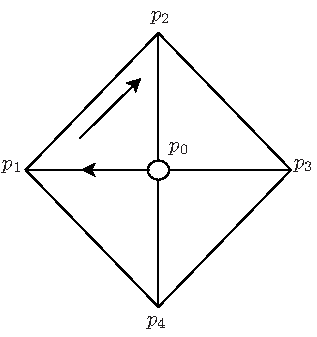
\includegraphics[width= 0.3\textwidth]{Figures/fp}
\caption{Strategy for the fixed flight plan}
\label{f:fp}
\end{figure}

The basic logic of how it works is explained as follows:
Suppose the \ac{UAV} always starts from waypoint $p_0$. If it does not start from $p_0$, set $p_0$ as the stand by waypoint. Design four blocks which are denoted as ``go $p_1$'', ``go $p_2$'', ``go $p_3$'' and ``go $p_4$'' respectively. 

While executing the four blocks, it also executes an exception condition. Suppose the \ac{UAV} starts from $p_0$, now it goes to $p_1$. During this process, it will also run 
the following exception conditions:
\begin{enumerate}
\item if $\psi_v<0$, execute ``go $p_4$''.
\item if $\psi_v>0$, execute ``go $p_2$''.
\end{enumerate}
%
where $\psi_v$ is the heading angle generated by the vision algorithm.
If the \ac{UAV} is going from $p_1$ to $p_2$, then it also executes the following exception conditions:
\begin{enumerate}
\item if $\psi_v<0$, execute ``go $p_1$''.
\item if $\psi_v>0$, execute ``go $p_0$''.
\end{enumerate}




\subsection{Comparison and Choice of Flight plan}
\textcolor{red}{Comparison and discussion.}

\section{Simulation}
\label{section:simulation}
\subsection{Linear Simulation}
\label{subsec:lin_sim}
%\textcolor{red}{Yazdi's method and results}
In order to grasp the concept of the computer vision, a linear simulation program is developed in MATLAB. The simulation program is also used to preliminary test the chosen strategy before the code implementation into the paparazzi system.  

\subsubsection{Model and Setup}
\textbf{The tournament field} is modeled based on our observation of the cyberzoo and the rules stated in the first announcement of the tournament, as shown in three example in Figure\ref{f:TopViewSamples}.

\textbf{Poles}, our initial assumption of the possible obstacle, are placed inside the obstacle field. Since there are no setup information, we choose to randomize the pole initial parameters, i.e., the pole number, the pole diameter and the x-y position, as shown in the table\ref{t:RandomPole} below. The ranges of position (x,y) are set to make the whole body of a pole to always be inside the obstacle area, considering the diameter ranges. Each pole are always separated by at least a certain distance, which is assumed to be 2 times the diameter of the drone. The height of the pole is assumed  to be constant of 2 meters. 

\begin{table}
\caption{Range of pole parameters randomization in the linear simulation}
\label{t:RandomPole}
\begin{center}
\begin{tabular}{lcc}
\hline \hline
Parameter & Range & Unit \\\hline
Pole number & 4 - 10 & - \\
Diameter & 40 - 60 & cm \\
Positions (x,y) & 2.1 - 7.9 $^*$ & m \\\hline\hline
\end{tabular}
\end{center}

\end{table}

\textbf{The Drone} is modeled from the observation of the AR-drone quad-rotor. Four circles with a heading indicator is used to visualized the drone with diameter of 0.4 m, in a top-down view as shown in Figure~\ref{f:TopViewSamples}. The drone motion is modeled using only linear kinematic equations with velocity changes, treating the drone as a point mass. Heading orientation is added to support the camera-view model. The model also consist of a random addition to simulate Drone drifting in the real life. 

\textbf{Camera-view} is modeled based on the pin-hole camera model, coupled with the specification of the AR-drone front camera. The result can be observed, from a random position of obstacle, in Figure~\ref{f:CameraViewSamples}. Further calibration is conducted to match the result with the sample pictures (Figure~\ref{f:Calibrations}) taken from zero altitude with a pole positioned 0.5, 1 and 2 meters infront of the camera, resulting in a field of view of 44 degree vertically, and 77 degree horizontally, as also shown by the dashed line coming from the front of the drone, in the top-down view Figure~\ref{f:TopViewSamples}. 

\begin{figure}[h]
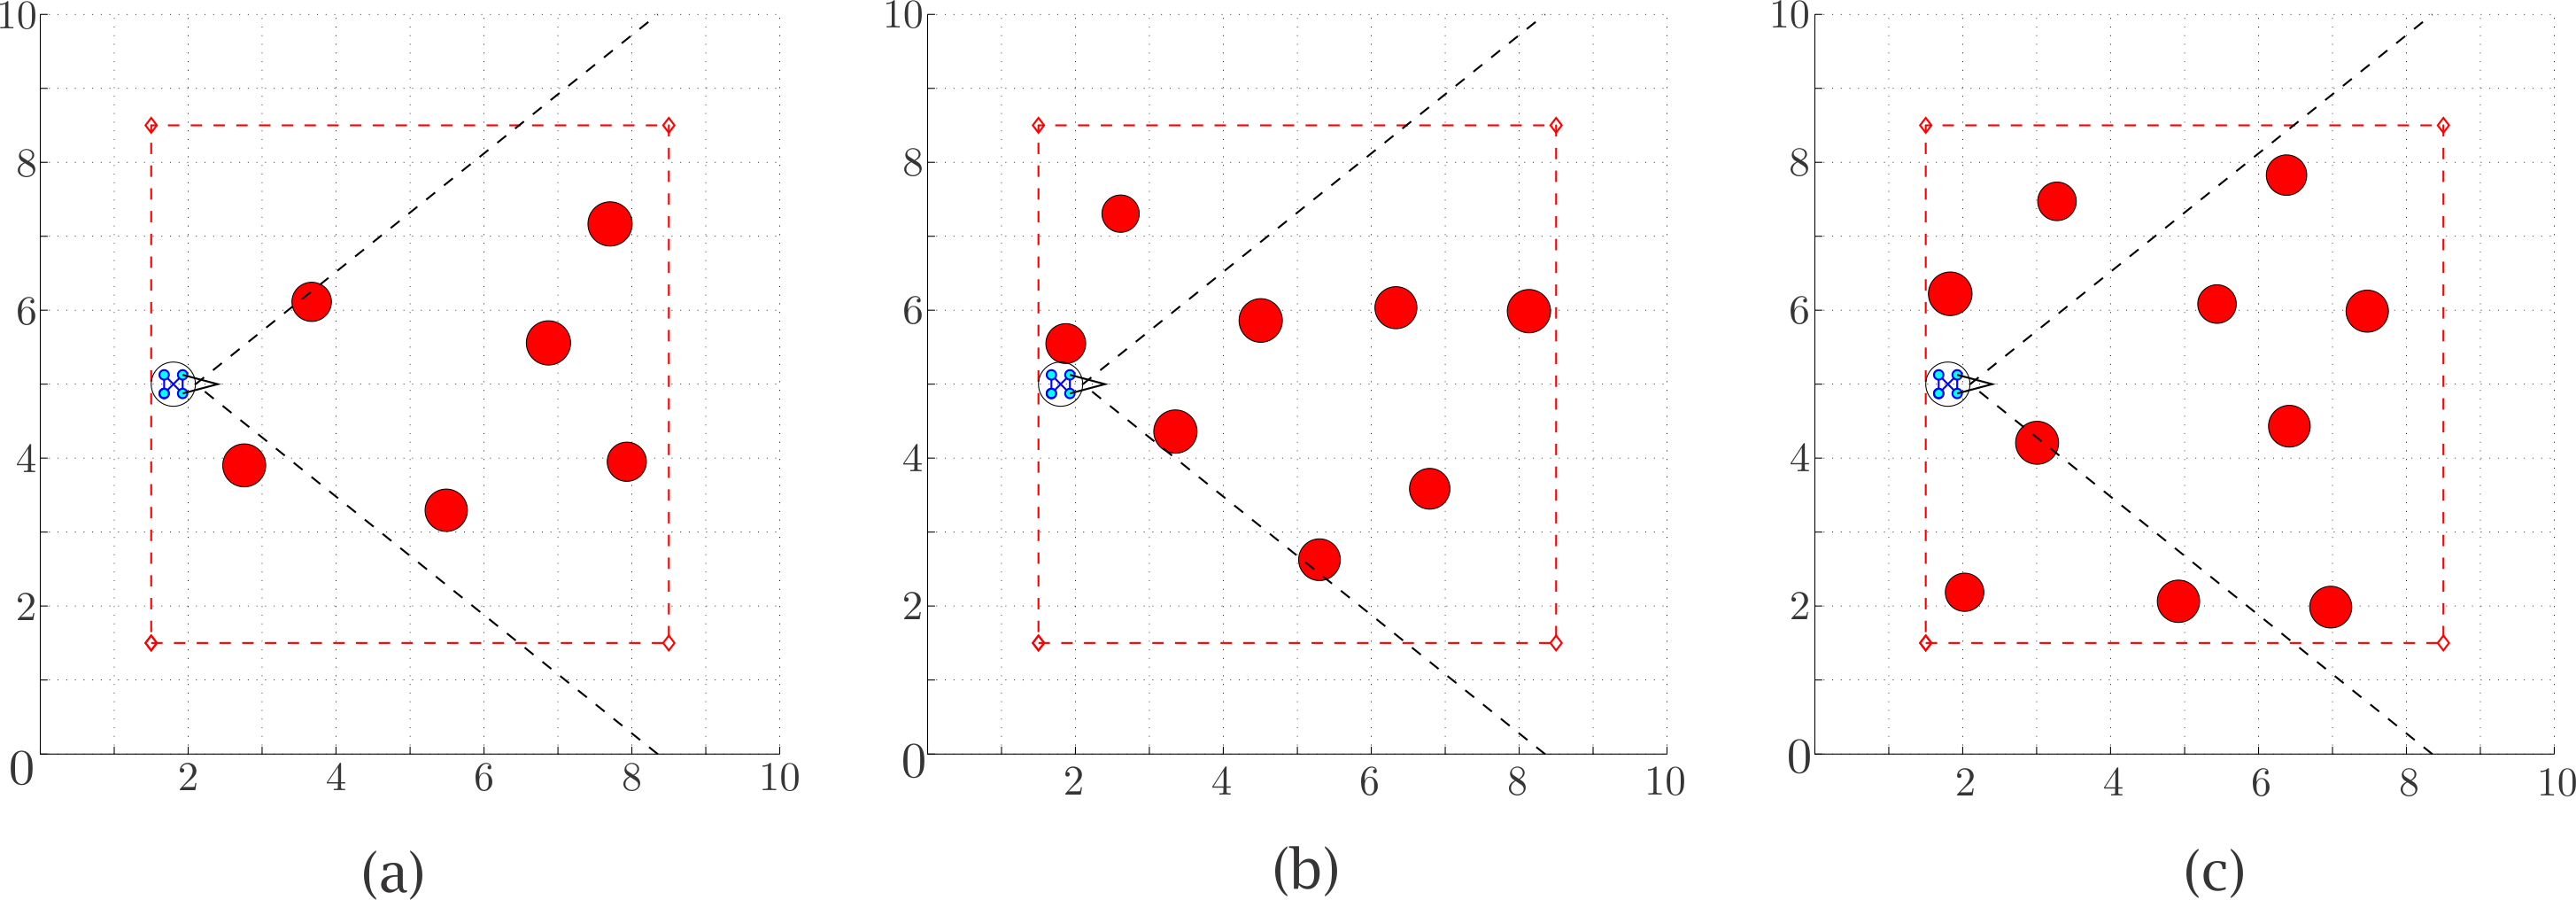
\includegraphics[width=1\linewidth]{Figures/TopViewSamples_3.png}
\centering
\caption{Three sample of obstacle random positioning in the competition field (cyberzoo), (a) with six poles, (b) with eight poles, and (c) with ten poles}
\label{f:TopViewSamples}
\end{figure} 

\begin{figure}[h]
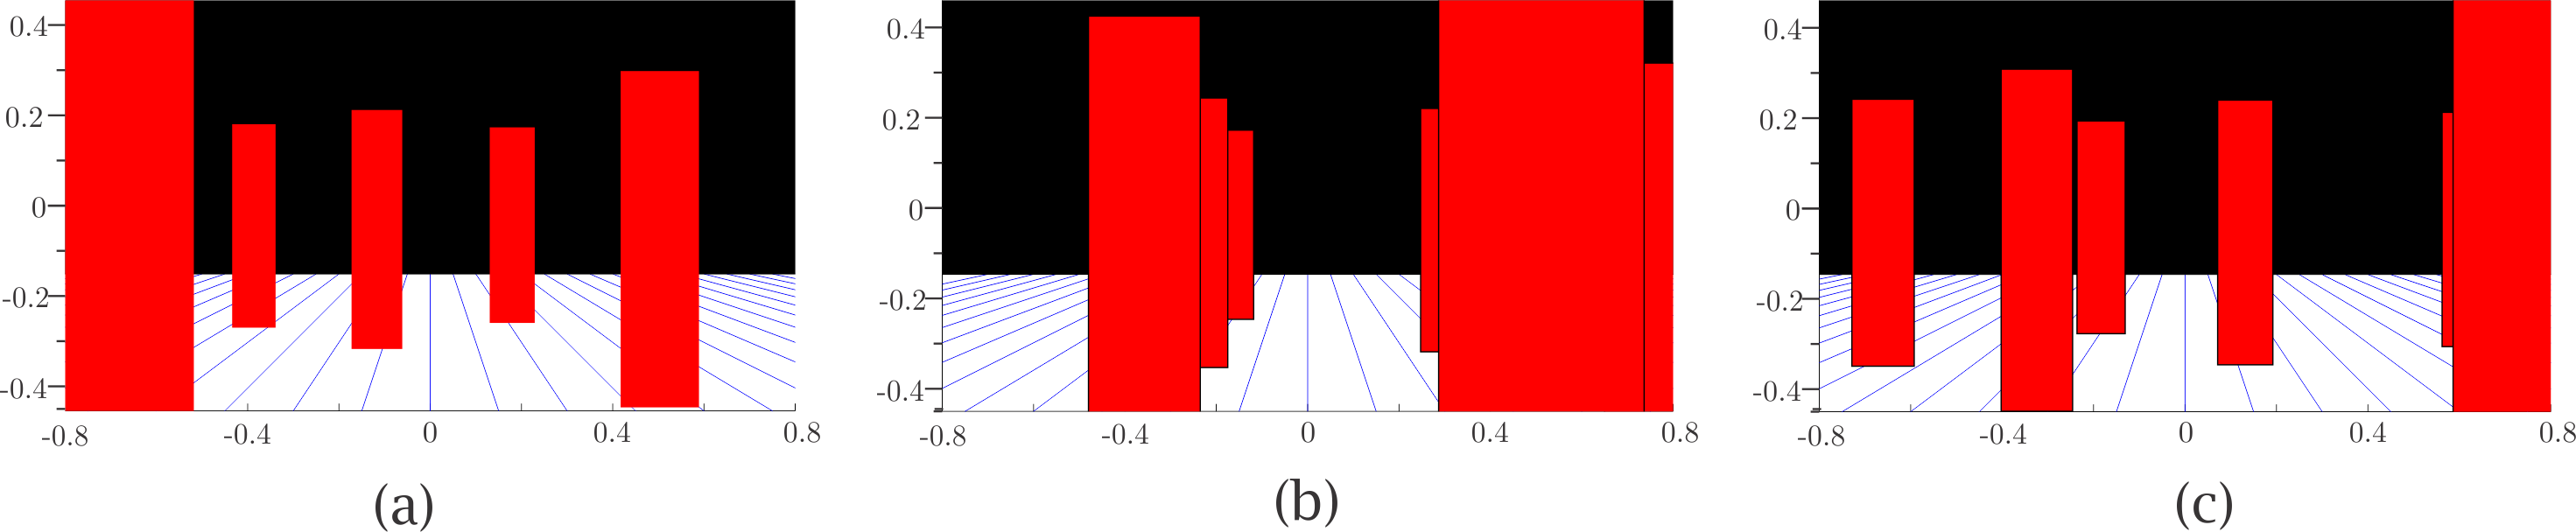
\includegraphics[width=1\linewidth]{Figures/CameraViewSamples_3.png}
\centering
\caption{Poles position as viewed by the AR.Drone front camera for (a) six poles, (b) eight poles, and (c) ten poles, corresponded to the sample (a), (b) and(c) in Figure~\ref{f:TopViewSamples}. Notice that not all poles are covered by the camera field-of-view (FOV)}
\label{f:CameraViewSamples}
\end{figure} 

\begin{figure}
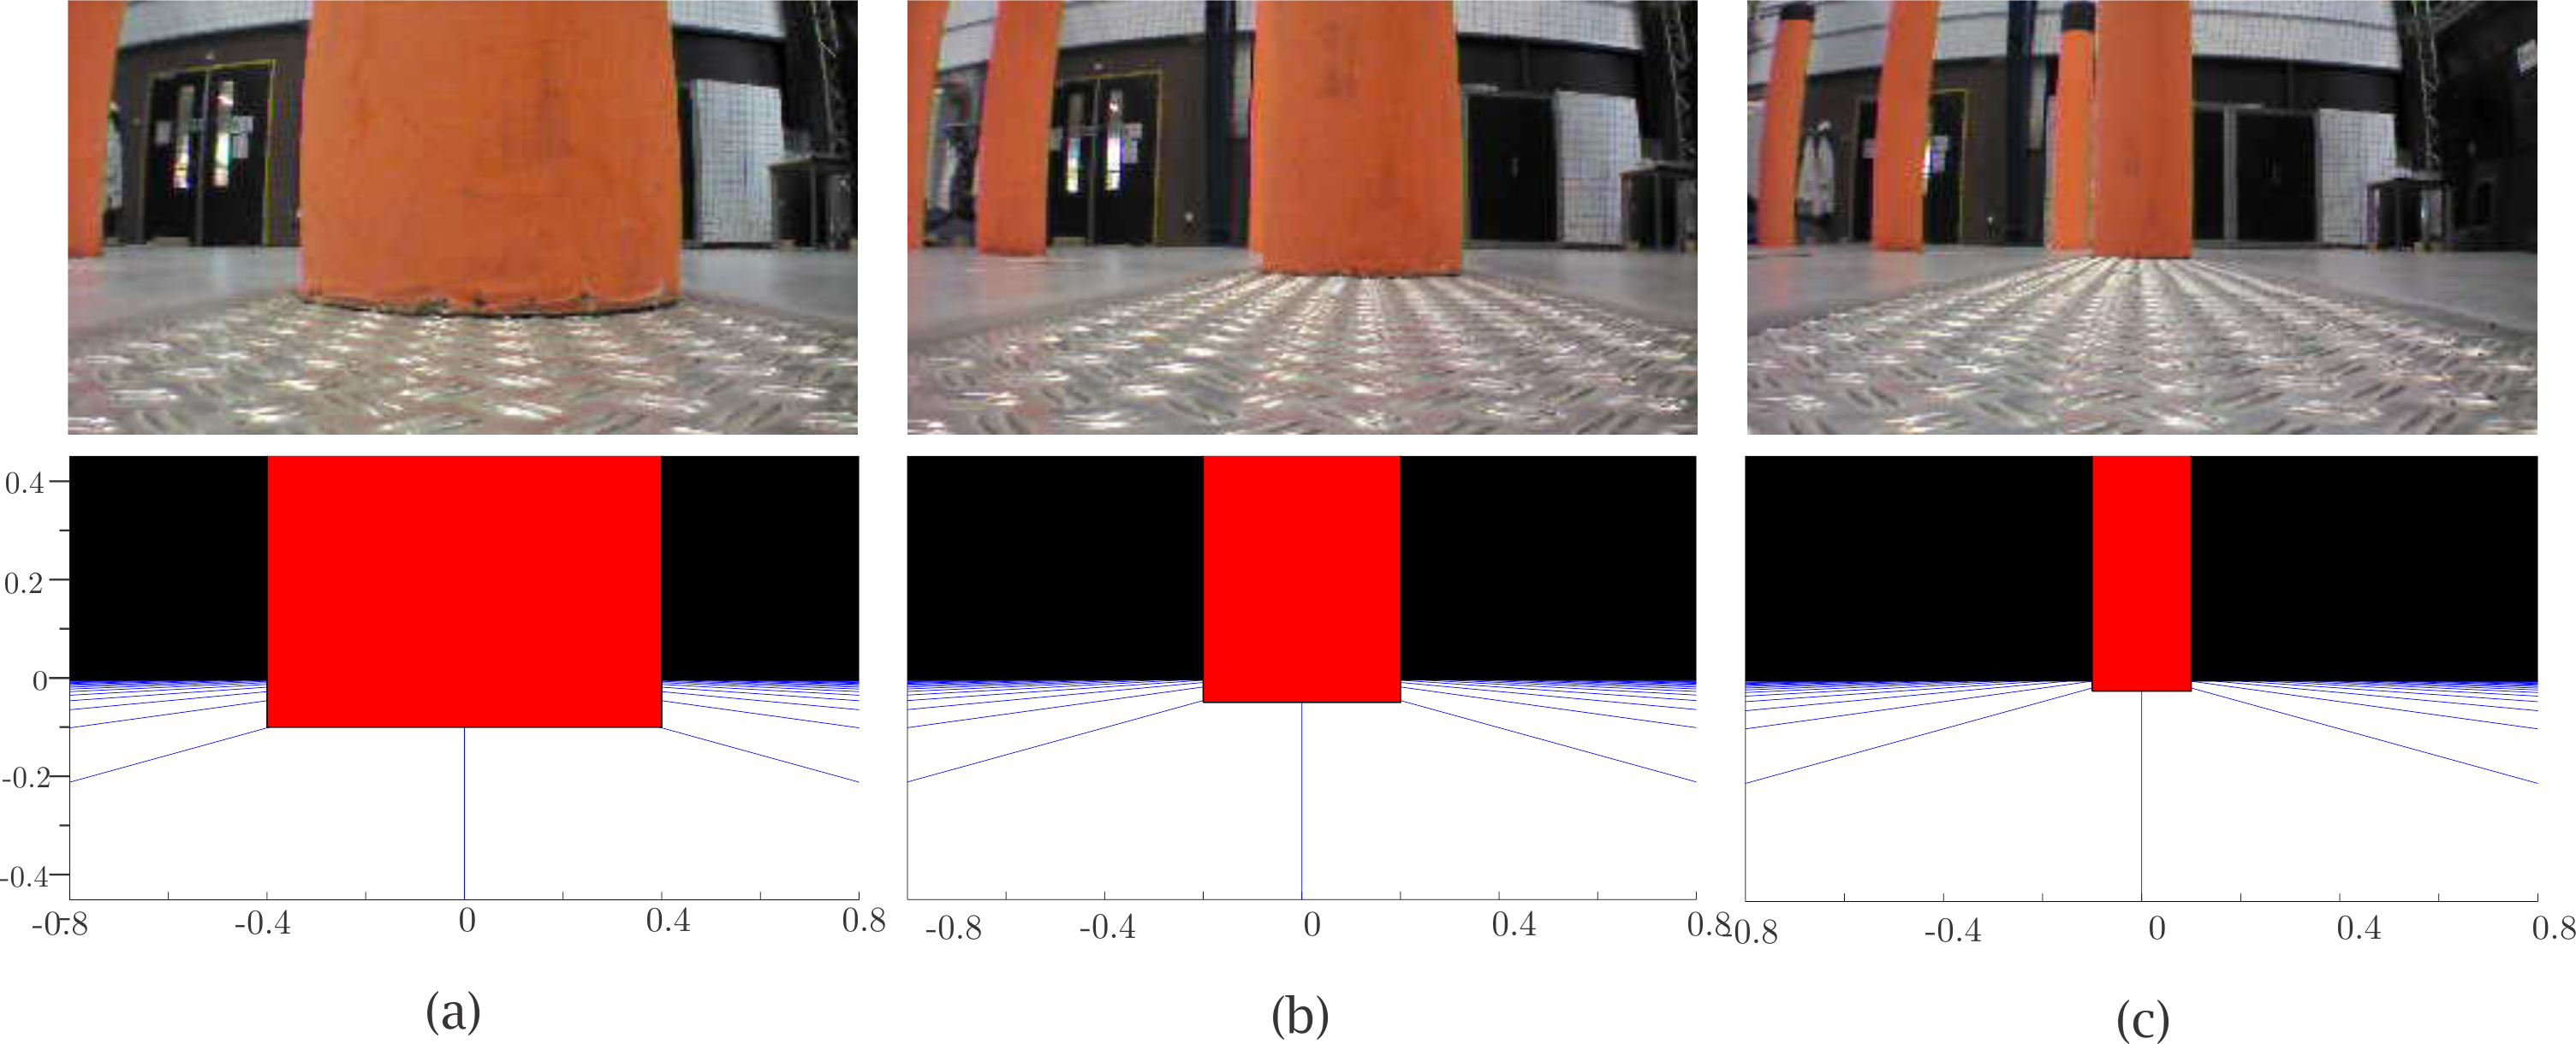
\includegraphics[width=1\linewidth]{Figures/Calibrations.png}
\centering
\caption{Calibration of the camera view model, conducted by comparing real snapshots from the AR.Drone front camera (top) with the result in the simulation (bottom). The drone on ground and a pole is positioned at (a) 0.5 meter, (b) 1 meter, and (c) two meter from the front camera.}
\label{f:Calibrations}
\end{figure} 



\subsubsection{Strategy Implementation Result}
The implemented strategy is as described in the previous section, summarized in the flow chart in Figure~\ref{fp1}. The result is shown in series of frames (time-captured) as can be observed in Figure~\ref{f:Simulation_8Poles}, for the situation where eight poles is used. The first strategy is tested in random obstacle configuration in the tournament field. It should be noted that the result shown in this report is not the best result for the strategy proposed, since it result in four collisions. Tuning of thresholds is required, which unfortunately have not been conducted thoroughly in this simulation due the limitation of time.

\begin{figure}[h]
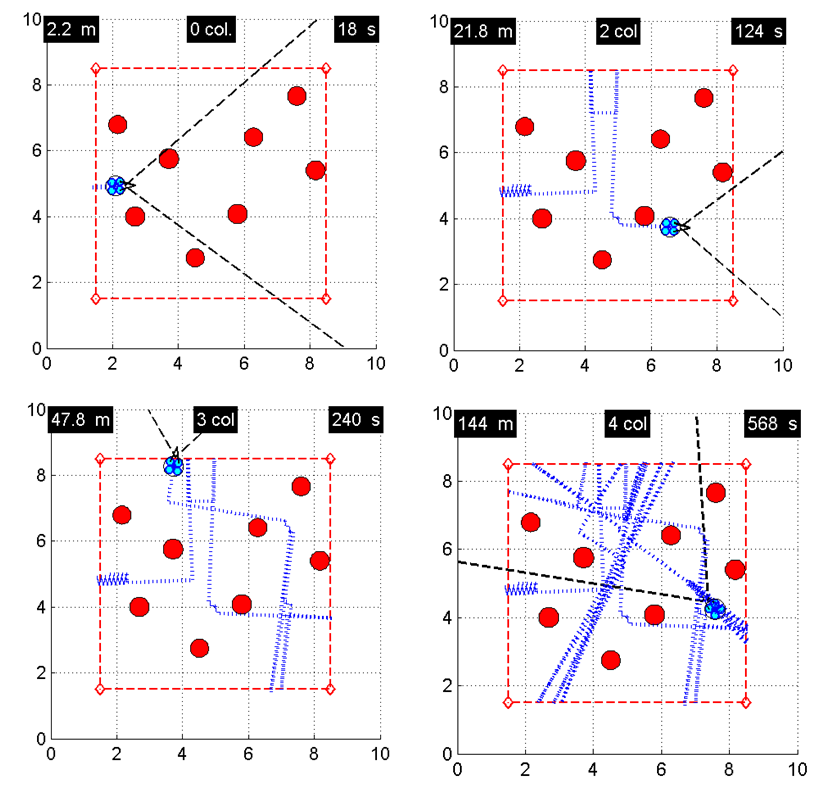
\includegraphics[width=1\linewidth]{Figures/Simulation_8Poles.png}
\centering
\caption{Simulation runs for 10 minutes, for cases with eight poles positioned in random.}
\label{f:Simulation_8Poles}
\end{figure}



\subsection{MATLAB \& Paparazzi Simulation}
Another way to carry out a simulation is to use MATLAB for the simulation of the vision algorithm (see Figure \ref{matlab}), and Paparazzi NPS simulator for the simulation of the flight plan (see Figure \ref{paparazzi_sim}). From the MATLAB simulation results, the appropriate color and width-thresholds for the initial practical trial can be derived. Note that these thresholds can only serve as the initial values because in the end they have to be fine-tuned through real-life tests. As for the flight plan, the Paparazzi NPS simulator can be used to verify the practicability and performance of the proposed flight plan. Although this simulator can yield realistic results, it has a drawback that the simulation cannot incorporate the vision algorithm. Thus, a "fake vision result" is supplied by an NPS file which we designed as a random number generator; it gives 0, 1, and -1 as output where 0 means 'no obstacle detected', 1 means 'obstacle on the left', and -1 means 'obstacle on the right'. The frequency of the occasions when it gives 1 or -1 is adjusted in this NPS file, so that by increasing this frequency, the simulation represents the situation where there are many obstacles present.
\begin{figure}[h]
	\centering
	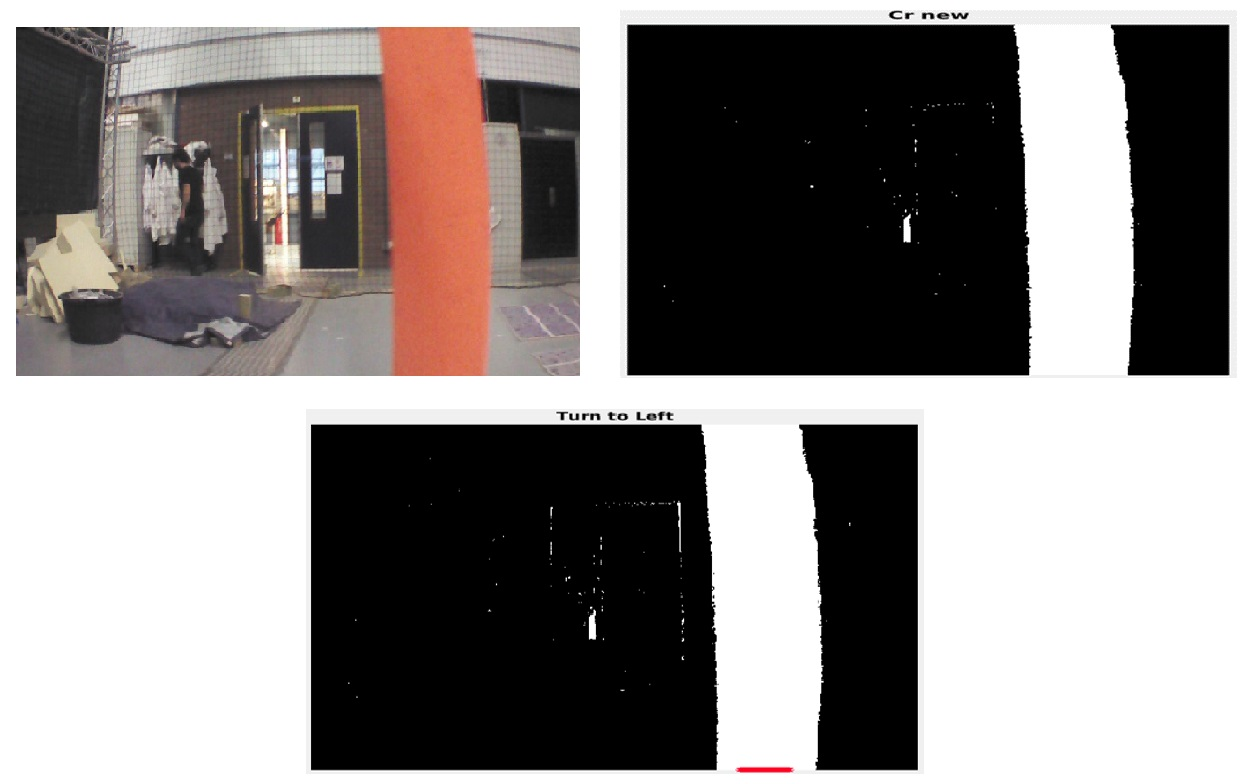
\includegraphics[width = 0.5\textwidth]{Figures/matlab.jpg}
	\caption{MATLAB simulation of vision algorithm using an image from the AR.Drone 2.0. Top left: original image captured. Top right: binary map computed using a threshold in Cr channel. Bottom: Detection of the orange pole. The red marks on the bottommost row indicate the location of the orange pole nearby.}
	\label{matlab}
\end{figure}
\begin{figure}[h]
	\centering
	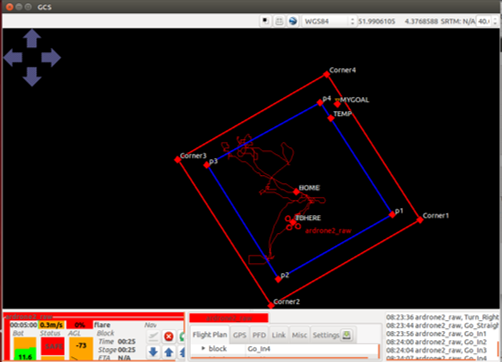
\includegraphics[width = 0.5\textwidth]{Figures/paparazzi_sim.png}
	\caption{Paparazzi simulation of the flight plan. The blue lines indicate the boundaries of the flight area.}
	\label{paparazzi_sim}
\end{figure}

\section{Competition Result and Discussion}
After tuning the control and vision threshold parameters through trial-and-error in real tests, it was confirmed that both vision algorithm and flight plan works very well with adequate sensitivity towards the distance from the orange poles and black wall. Also, it was observed that the drone could maintain a stable flight during the maneuvers, such as stopping and turning of the heading. The slow speed of the drone, together with the intermittent turning strategy, allowed the drone to stop and turn with only a marginal overshoot whenever an obstacle is detected or it goes outside the flight area. Regrettably, however, the tuning was done in the environment where the obstacles were rather spaced out widely, and in particular, the black wall was positioned near and parallel to one of the boundaries of the flight area.\\

During the actual competition, the black wall was positioned adjacently near one of the corners, and there was another orange pole next to it. What happened in the first half of the competition was: the drone moved and made a few turns, and eventually went to near the corner. After it realized that it was out of bounds, it made $180^o$ turn and attempted to come back inside. However it saw the adjacent black wall, and turned to the other side. Then it saw the orange wall and turned back to the previous heading. And it saw the black wall again, and so on. After drifting slowly towards the black wall, it touched the black wall and had to be restarted due to the low battery.\\

In the second half of the competition, the drone was started after being repositioned in the home position, so it did not go into the corner and did not get trapped again. As a result, the drone covered the traveled distance of well more than 100 m. Although this is not quite a high result compared to the other teams, our drone had the fewest collisions with the obstacle, and our team won the 6th place out of 13 teams in total.\\

In the following list, the main reasons are addressed as to why it could not be foreseen that the drone may get trapped near the boundaries/corners:
\begin{itemize}
	\item In the Paparazzi simulation, the vision algorithm was "mimicked" by a random number generator. Hence, there was never a possibility of a drone getting trapped in a place.
	\item During the real tests for tuning, the black wall was located parallel to one of the boundaries and further way from the corner. So, the drone could not be possibly trapped by the "blocking" of the wall.
\end{itemize}

To solve this problem in the future, the following strategies may be used to improve the flight plan:
\begin{itemize}
	\item "Breakthrough Maneuver": Incorporate a maneuver that when a drone makes more than two consecutive turns back and forth, turn the heading only $45^o$ and fly forward for a certain period of time while suppressing command from the vision result.
	\item "Temporary Blinding": In case the displacement of the drone is too low during a fixed time period, flexibly adjust the vision threshold parameters (e.g. the width threshold for the pole detection) such that the drone becomes less sensitive towards the obstacles nearby.
	\item "Circular Flight Area": Define the flight area as a circle, instead of a square. This will prevent the drone from going too close into a corner.
\end{itemize}

\section{Conclusion}
The performance of the AR.Drone in the competition validates both the proposed vision algorithm and the flight plan. This team drone was able to maintain a stable flight throughout the whole ten minutes without any major collision. Although two minor collision and one down time did occur, there are both due to circumstances that was not part of the algorithm design objectives. In the end our drone manage to have the fewest collision from all other team that manage to fly their drone. However, the drone only secure the 6th position out of 13 teams, due to the short covered distance. This distance result are actually confirms what the simulations before the competition suggested. However, beside the black wall trapping, we did not think that a distance more than 100 meter is actually too short in the competition that have minimum distance threshold of 40 meter, that we decide to fly the drone as slow for stability. 

Several strategies might be implemented in the future to achieve higher score in a competition, such as a Breaktrough Maneuver, Temporary Blinding, or Circular Flight Area. Adjusting the speed of the drone is also an option to have more covered distance. Overall, the competition was held well and could be a very good method to gain experience in flying an MAV autonomously, especially in preparation of the real IMAV competition



% BIBLIOGRAPHY:
% use {unsrt}:
\bibliographystyle{unsrt}
\bibliography{imav_bibliography}

% The following lines are necessary for showing the appendices correctly, do not change!
\appendix
\newcommand{\appsection}[1]{\let\oldthesection\thesection
  \renewcommand{\thesection}{Appendix \oldthesection:}
  \section{#1}\let\thesection\oldthesection}
% appendices are now indicated by appsection:

%\appsection{Data}
%\appsection{More data}
\end{document}

